%%%%%%%%%%%%%%%%%%%%%%%%%%%%%%%%%%%%%%%%%%%%%%%%%%
\section{Analysis Description}
%%%%%%%%%%%%%%%%%%%%%%%%%%%%%%%%%%%%%%%%%%%%%%%%%%

%-------------
The analysis is designed for maximum sensitivity to the T2tt model resulting in final states with many light-flavour jets, b-tagged jets, no leptons, and large \MET. 
%
Targeting the above-mentioned final states, data are initially selected by requiring a number of jets and b-jets (\njets and \nbjets) and a large \MET. 
%
The search regions are ultimately defined in exclusive bins of \ntops, \nbjets, \MET and a kinematic variable \MTTwo, defined in Sec.~\ref{sec:searchregions}. SM backgrounds come from processes such as QCD multijet events, Z bosons produced in association with jets (Z+jets), top quarks or W bosons produced in association with jets (t/W+jets), and smaller contributions from rare SM processes.
%
%The top reconstruction and identification procedure (top tagging) is described in this section, as well as the Monte Carlo (MC) samples that model signal and backgrounds.
%
%The data selection process starts with the trigger requirements and follows with a pre-selection and the definition of the search bins. 

%%%%%%%%%%%%%%%%%%%%%%%%%%%%%%%%%%%%%%%%%%%%%%%%%%
\subsection{Top quark reconstruction and identification}
%%%%%%%%%%%%%%%%%%%%%%%%%%%%%%%%%%%%%%%%%%%%%%%%%%

%-------------
The procedure to reconstruct and identify the hadronically-decaying top quarks (top-tagging) in the 2015 13~TeV analysis is similar to the one used in Ref.~\cite{stop8TeV}, where reconstruction of the hadronically decaying top quarks is performed as described in Refs.~\cite{Kaplan:2008ie,Plehn:2010st,Kaplan:2012gd}.  
%
The collection of four or more jets from events in the pre-selection sample is divided into all possible sets of three jets and a remnant system, where the remnant system must contain at least one b-tagged jet. 
%
The fully reconstructed top quark is one of the three-jet (trijet) combinations. 
%
To be considered as a fully reconstructed top quark, the trijet system must satisfy the following requirements. 
%
(i) Each jet lies within a cone of radius 1.5 in ($\eta,\phi$) space, centered at the direction defined by the trijet combination. 
%
The radius requirement implies a moderate Lorentz boost of the top quark as expected for events with large $\Delta m = m_{\sTop} - m_{\chiOneZero}$ targeted in this search.
%
(ii) The trijet system mass ($m_{\text{3-jet}}$) must be within the range 100-250~\GeVcc.
%
(iii) The trijet system must satisfy one of the three following criteria:
\begin{equation} \label{eq:taggerEQ}
   \begin{array}{l}
     \displaystyle{
     \mbox{a)}~~ 0.2< \arctan\left(\frac{m_{13}}{m_{12}}\right) < 1.3 ~~\mbox{and}~~ R_\mathrm{min} < \frac{m_{23}}{m_{\text{3-jet}}} < R_\mathrm{max}}, \\
     %%
     \displaystyle{
     \mbox{b)}~~ R_\mathrm{min}^{2}\left(1+\left(\frac{m_{13}}{m_{12}}\right)^2\right) 
     < 1-\left(\frac{m_{23}}{m_{\text{3-jet}}}\right)^2 
     < R_\mathrm{max}^{2}\left(1+\left(\frac{m_{13}}{m_{12}}\right)^2\right) ~~\mbox{and}~~ \frac{m_{23}}{m_{\text{3-jet}}} > 0.35}, \\
     %%
     \displaystyle{
     \mbox{c)}~~ R_\mathrm{min}^{2}\left(1+\left(\frac{m_{12}}{m_{13}}\right)^2\right) 
     < 1-\left(\frac{m_{23}}{m_{\text{3-jet}}}\right)^2 
     < R_\mathrm{max}^{2}\left(1+\left(\frac{m_{12}}{m_{13}}\right)^2\right) ~~\mbox{and}~~ \frac{m_{23}}{m_{\text{3-jet}}} > 0.35}. \\
   \end{array} 
\end{equation}
%
Here, $m_{12}$, $m_{13}$, and $m_{23}$ are the dijet masses, where the jet indices 1, 2, and 3 are \pt ordered.
%
The following numerical constants have values $R_\mathrm{min} = 0.85\cdot(m_{\W}/m_{\mathrm{\topquark}})$, $R_\mathrm{max} = 1.25\cdot(m_{\W}/m_{\mathrm{\topquark}})$, $m_{\W} = 80.4$~\GeV, and $m_{\mathrm{\topquark}} = 173.4$~\GeV~\cite{PDG}.
%
The top-quark tagging (t-tagging) conditions of a), b), or c) can be reduced (under certain approximations detailed in Ref.~\cite{Plehn:2010st}) to the requirement that $m_{23}/m_{\text{3-jet}}$, $m_{12}/m_{\text{3-jet}}$, or $m_{13}/m_{\text{3-jet}}$, respectively, be consistent with the $m_{\W}/m_{\mathrm{\topquark}}$ ratio.
%
The other conditions are motivated by the Lorentz structure of the tW coupling and suppress contributions from light-quark and gluon jets~\cite{Plehn:2010st}. 
%
If multiple trijet combinations satisfy these criteria, the triplet with mass closest to the top quark mass is selected.

%-------------
The top-tagging algorithm is improved in this work, compared with ~\cite{stop8TeV}, to be sensitive to boosted senarios where decay products from the $W$ boson or top quark are merged.  
%
Specifically, the jet mass is used to determine if the jet represents the merged decay products of a $W$ boson (merged $W$ jet) or a top quark (merged top jet).  
%
When the jet mass is in the 70-110 \gev range, it is considered as a $W$ boson, and a top quark when it is in the 110-220 \gev range.
%
Once a merged $W$ boson jet is identified, an additional jet is combined with it to form a potential top candidiate. 
%
The merged $W$ boson jet is treated as a ``dijet'' system in the top tagging algorithm, and  $R_{min} < m_W/m_{W+j} < R_{max}$ is used as a criteria to decide if it is a good top candidate. 
%
In case a single jet is identified as a top quark jet, it is simply treated as a top candidate. 
%
For merged top quark jets, the tagger has good efficiency over a wide range of top quark \pt, from $\sim25\%$ at 200 \gev to close to 80\% at 1~TeV. 

%%%%%%%%%%%%%%%%%%%%%%%%%%%%%%%%%%%%%%%%%%%%%%%%%%
\subsection{Trigger path}
\label{sec:trig}
%%%%%%%%%%%%%%%%%%%%%%%%%%%%%%%%%%%%%%%%%%%%%%%%%%

%-------------
Events in the search regions, as well as the single-lepton and multijet samples for electroweak and QCD background estimations are collected from a Level 1 hardware trigger which applies a threshold on the scalar summed transverse energy over all (calorimeter-only) jets in the event of at least 175~\GeV. 
%
If the event is accepted, the high-level trigger then requires a calorimeter-based \HT $>280$ \gev and a calorimeter-based \met $>70$ \gev.  
%
Finally, the high-level trigger applies a threshold on the scalar summed transverse momenta (\HT) over all particle flow based jets in the event of greater than 350~\GeV in coincidence with a threshold on the missing transverse momentum (\MET) above 100~\GeV computed using all particle flow candidates in the event.  
%
Studies show that this analysis is fully efficient, if one requires at least 175~\GeV of particle-flow based \MET together with at least 500~\GeV of particle-flow based $H_{\rm T}$.

%%%%%%%%%%%%%%%%%%%%%%%%%%%%%%%%%%%%%%%%%%%%%%%%%%
\subsection{Pre-selection}
\label{sec:pre-selection}
%%%%%%%%%%%%%%%%%%%%%%%%%%%%%%%%%%%%%%%%%%%%%%%%%%

%-------------
The search looks for multijet events, with b-jets decaying from top quarks, large \MET and no leptons. 
%
Initially, a loose pre-selection selection is applied in \MET, \njets and \nbjets, which preserves 2-20\% of the signal events. 
%
The events passing the pre-selection selection are then later classified into search regions. 
%
The following criteria define the pre-selection selection.

%-------------
All events must pass filters designed to remove detector- and beam-related noise.  
%
All jets considered in this analysis are required to have $\pt>$30 \gev and $|\eta|<$2.4.  
%
In addition, all jets must pass a set of ``loose'' jet identification criteria. 
%
The minimum number of such jets in an event must be $\njets\geq4$, with the leading two jets required to have $\pt>$50 \gev.  
%
The missing transverse momentum must satisfy \MET $\ge$ 200 \gev, where the threshold is chosen so as to be well on the trigger efficiency plateau and also to allow a low 175~\GeV $\<$ \MET sideband for background studies.  
%
The scalar summed transverse momentum of the event must satisfy \HT $\ge$ 500 \gev, with \HT = $\sum_{\mathrm{jets}} \pt$, also chosen to be on the trigger efficiency plateau.  
%
Jets in the \HT calculation must meet the same jet seletion criteria defined above.  
%
The number of heavy-flavor tagged jets in the event must satisfy \nbjets $\ge$ 1, with b-jets identified using the CSV b-tagging algorithm (CSVM), medium working point.
%
Events are vetoed if they contain isolated muon candidates that satisfy $\pt>$10 \gev and $|\eta|<$2.4.
%
A relative-isolation criteria is enforced for which an isolation cone shrinks as a function of increasing muon \pt. 
%
The \pt in the shrinking cone is required to be less than 20\% of the muon \pt. 
%
Events are further vetoed if the contain isolated electron candidates that have $\pt>$10 \gev and $|\eta|<$2.5. 
%
Isolated electrons are determined using a similar isolation requirement as for muons, except that less than 10\% of the electron energy is required to be in the shrinking isolation cone.
%
A requirement on the angle between \MET and the first three leading jets, $\Delta\phi(\MET, j_{1,2,3})>$ 0.5, 0.5, 0.3, is applied to remove events coming from QCD processes.
%
After applying the cuts described above the residual background comes from \ttbar, single top, and $W+$jets events with one $W\rightarrow l\nu$ decay where $l$ can be an electron, muon or tau decaying hadronically. 
%
To further suppress these backgrounds, we reject events that have one or more isolated tracks. 
%
The track isolation is calculated from charged PF candidates consistent with the reconstructed primary vertex ($|dz(PV)|<0.1~\mathrm{cm}$).
%
The requirements are different for muon, electron and charged hadron tracks.
%
For both electron and muon tracks, the isolated track requirements are: $\pt>$5 \gev, $|\eta|<$2.5 and a relative isolation of less than 0.2.
%
For charged hadron tracks, the \pt requirement is raised to be at least 10 \gev and the relative isolation value to be less than 0.1. 
%
To improve signal-to-background event discrimination, events with one isolated track, as defined above, are only rejected if they satisfy $m_T(tk,\met) = \sqrt{2p_{T}^{tk}\met(1-\cos\Delta\phi)}<100\;\mathrm{GeV}$, where $p_{T}^{tk}$ is the transverse momentum of the track and $\Delta\phi$ is the azimuthal separation between the track and \METv. 
%
Tables~\ref{tab:cutflowMC1},~\ref{tab:cutflowMC2} in Appendix~\ref{sec:appendixcutflow} illustrate the effect of the pre-selection cuts on background SM processes using MC simulation. Table~\ref{tab:cutflowMC3} in Appendix~\ref{sec:appendixcutflow} shows the effects of the pre-selection cuts on two example signal models.  

%%%%%%%%%%%%%%%%%%%%%%%%%%%%%%%%%%%%%%%%%%%%%%%%%%
\subsection{Search region selections}
\label{sec:searchregions}
%%%%%%%%%%%%%%%%%%%%%%%%%%%%%%%%%%%%%%%%%%%%%%%%%%

%-------------
We bin the search regions in terms of the number of b-tagged jets and top candidates. 
%
A top candidate is defined to be an object that satifies the top-tag criteria as shown in equation~\ref{eq:taggerEQ} with the QCD rejection cut removed ($m_{23}/m_{3-jet}>$0.35). 
%
If a top candidate is reconstructed in the event and a b-tagged jet identified in the remaining system (R-sys), this candidate is added first to the top counting list. 
%
Events with only one top candidate and no b-tagged jet in the R-sys are rejected.
%
Additional top candidates reconstructed from the R-sys are considered, starting from those with mass closest to the top quark mass. 
%
To avoid any two top candidates to share the same jets, we verify that the additional top candidate does not include a jet identified as part of an existing candidate. 
%
If it does, the additional candidate is discarded. 
%
Note that, as stated in Ref.~\cite{stop8TeV}, the top candidate definition has no explicit requirement on b-tagged jets. 
%
Thus there is not a one-to-one correspondence between the number of top candidates and the number of b-tagged jets in an event.  
%
The number of b-jets and top candidates variables are binned as $\nbjets=1$, $\nbjets=2$ and $\ntops=1$, $\ntops=2$. 
%
Exclusive search regions are defined for all combinations of \nbjets and \ntops bins.
%

%-------------
To improve background suppression, in particular the \ttbar contribution, the \MET and \MTTwo variables are added to the set that defines the search regions. 
%
The variable \MTTwo~\cite{Lester:1999tx,Barr:2003rg} is an extension of the transverse mass variable that is sensitive to the pair production of heavy particles, each of which decays to an invisible particle.
%
The \pTop, the \pRsystem, and the \MET in an event are used to constructed \MTTwo assuming the invisible particles are massless.
%
The \MTTwo variable is defined as:
%%%%%%%%%%%%%%%%%%%%%%%%%%%%%%%%%%%%%%%%%%%%%%%%%%
\begin{equation} \label{eq:MT2}
   \begin{array}{l}
     \displaystyle{ \MTTwo \equiv \min_{\vec{q}_{T}^{(1)}+\vec{q}_{T}^{(2)} = \vec{p}_{T}} [\max\{m_{T}^2(\vec{p}_{T}^{t^{(1)}}, \vec{q}_{T}^{(1)}; m_{\chi_1^0}), m_{T}^2(\vec{p}_{T}^{t^{(2)}}, \vec{q}_{T}^{(2)}; m_{\chi_1^0})\}]  } 
   \end{array}
\end{equation}
%%%%%%%%%%%%%%%%%%%%%%%%%%%%%%%%%%%%%%%%%%%%%%%%%%
where the $m_{T}^2$ is the transverse mass,
%%%%%%%%%%%%%%%%%%%%%%%%%%%%%%%%%%%%%%%%%%%%%%%%%%
\begin{equation} \label{eq:MTdef}
   \begin{array}{l}
     \displaystyle{
        m_{T}^2(\vec{p}_{T}^{t^{(1)}}, \vec{q}_{T}^{(1)}; m_{\chi_1^0}) \equiv m_{t^{(1)}}^{2} + m_{\chi_1^0}^2 + 2(E_{T}^{t^{(1)}}E_{T}^{(1)} - \vec{p}_{T}^{t^{(1)}} \cdot \vec{q}_{T}^{(1)})
     }
   \end{array}
\end{equation} 
%%%%%%%%%%%%%%%%%%%%%%%%%%%%%%%%%%%%%%%%%%%%%%%%%%
\MTTwo is a minimization of two transverse masses with a constraint that the sum of the transverse momenta of both $\chi_1^0$'s is equal to the missing transverse momentum of the event, i.e., $\vec{q}_{T}^{(1)}+\vec{q}_{T}^{(2)} = \vec{p}_{T}$. 
%
\MTTwo has a kinematic upper limit which is the \sTop mass. 
%
The superscripts $(1)$ and $(2)$ in the equations refer to the individual decays of the \sTop particles. 
%
In the specific case of the analysis described in this summary, we replace the quantities related to superscript $(1)$ by those of associated with the fully reconstructed top quark, i.e., the \pTop. 
%
Similarly, we replace the quantities related to superscript $(2)$ by those of the partially reconstructed top quark, i.e., the \pRsystem  for $\ntops =1$ and the fully reconstructed top quark for $\ntops \ge 2$. \MET then corresponds to $\vec{p}_{T}$ in the equation~\ref{eq:MT2}. 
%
Since we assume that the invisible particle is massless, $m_{\chi_1^0}$ should be zero in Eqs.~\ref{eq:MT2}-~\ref{eq:MTdef}. 

%-------------
We start from the fact that, by construction, there is always at least one hadronic top candidate in events that lie in the search bins. 
%
If there are two top candidates, \MTTwo is calculated using the pair of top candidates and \met. 
%
In the case of more than two top candidates, we compute \MTTwo for all combinations and choose the \MTTwo with the smallest value. 
%
If only one top candidate is identified by the top-tagging algorithm, we reconstruct the other top quark from the remanent of the event using the b-tagged jet as a seed and the R-sys jet closest to the b-tagged jet with an invariant mass between 50 \gev and the top quark mass. 
%
In case no R-sys jet combination satisfies that invariant mass requirement, we use the b-tagged jet as the only remanent of the other top quark. 
%
In the latter case, \MTTwo is calculated from the reconstructed top candidate, the remanent and the \met.

%-------------
Figure~\ref{fig:compSBvars} demonstrates the background composition following the pre-selection cuts and as a function of \ntops, \nbjets, \MET and \MTTwo, which are used to define the search bins.
%%%%%%%%%%%%%%%%%%%%%%%%%%%%%%%%%%%%%%%%%%%%%%%%%%
\begin{figure}[h]
  \begin{center}
    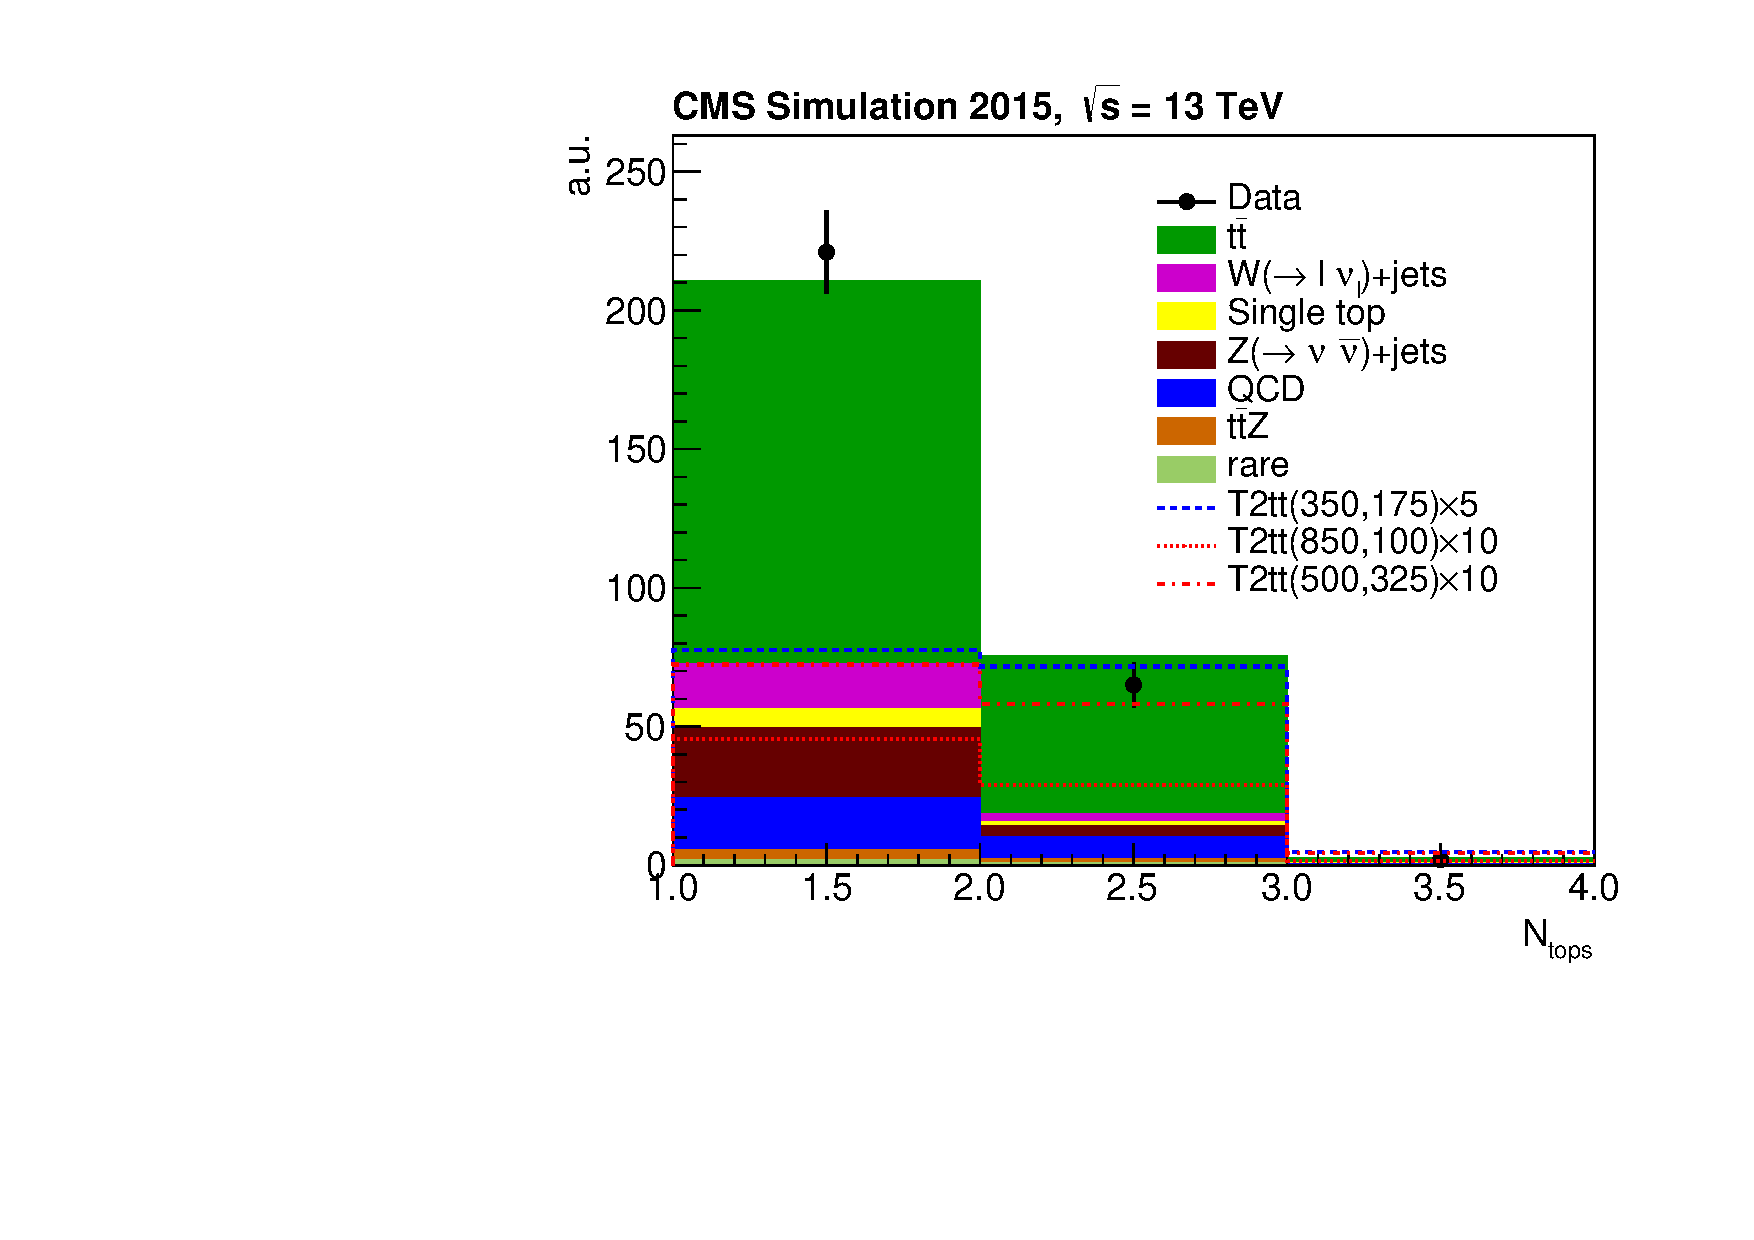
\includegraphics[width=0.48\linewidth]{figures/comb_nTops_baseline.pdf}
    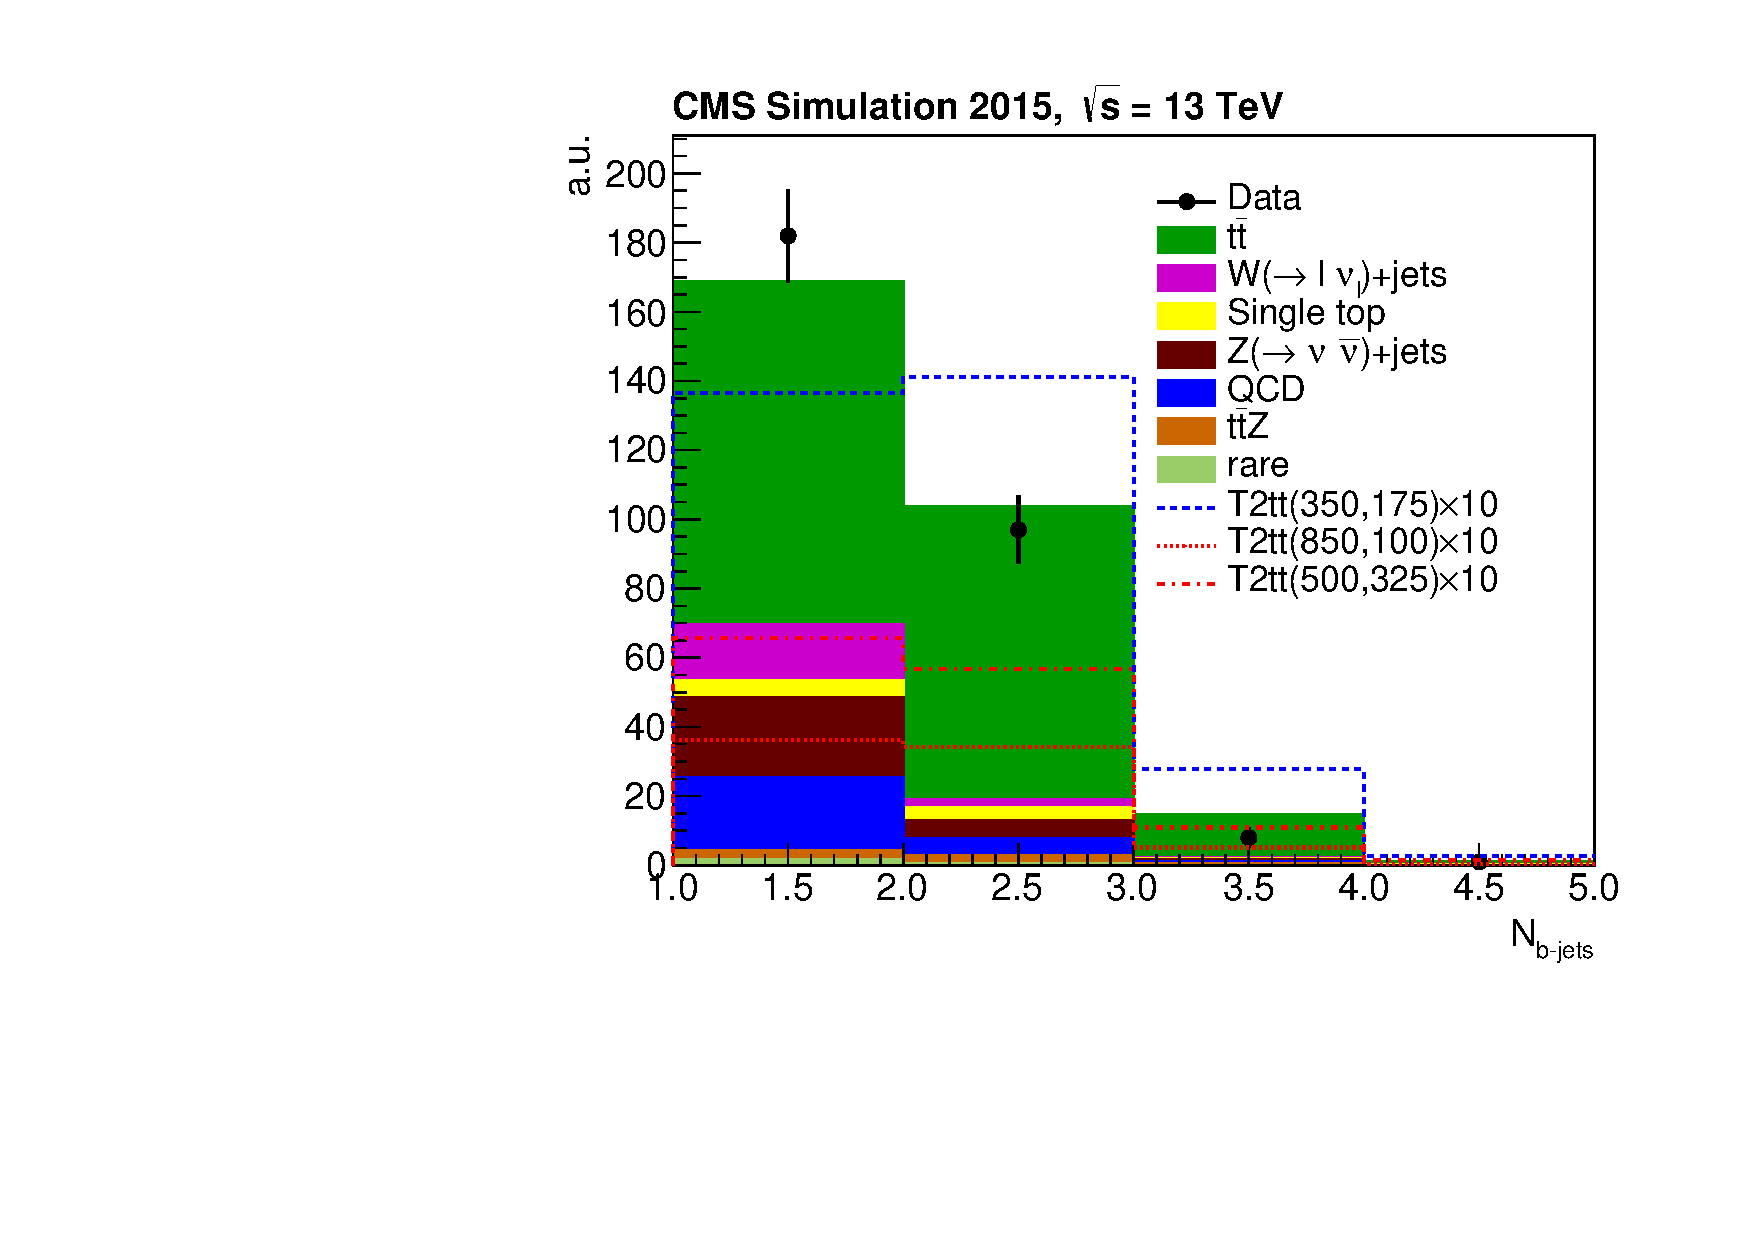
\includegraphics[width=0.48\linewidth]{figures/comb_nbJets_baseline.pdf} \\
    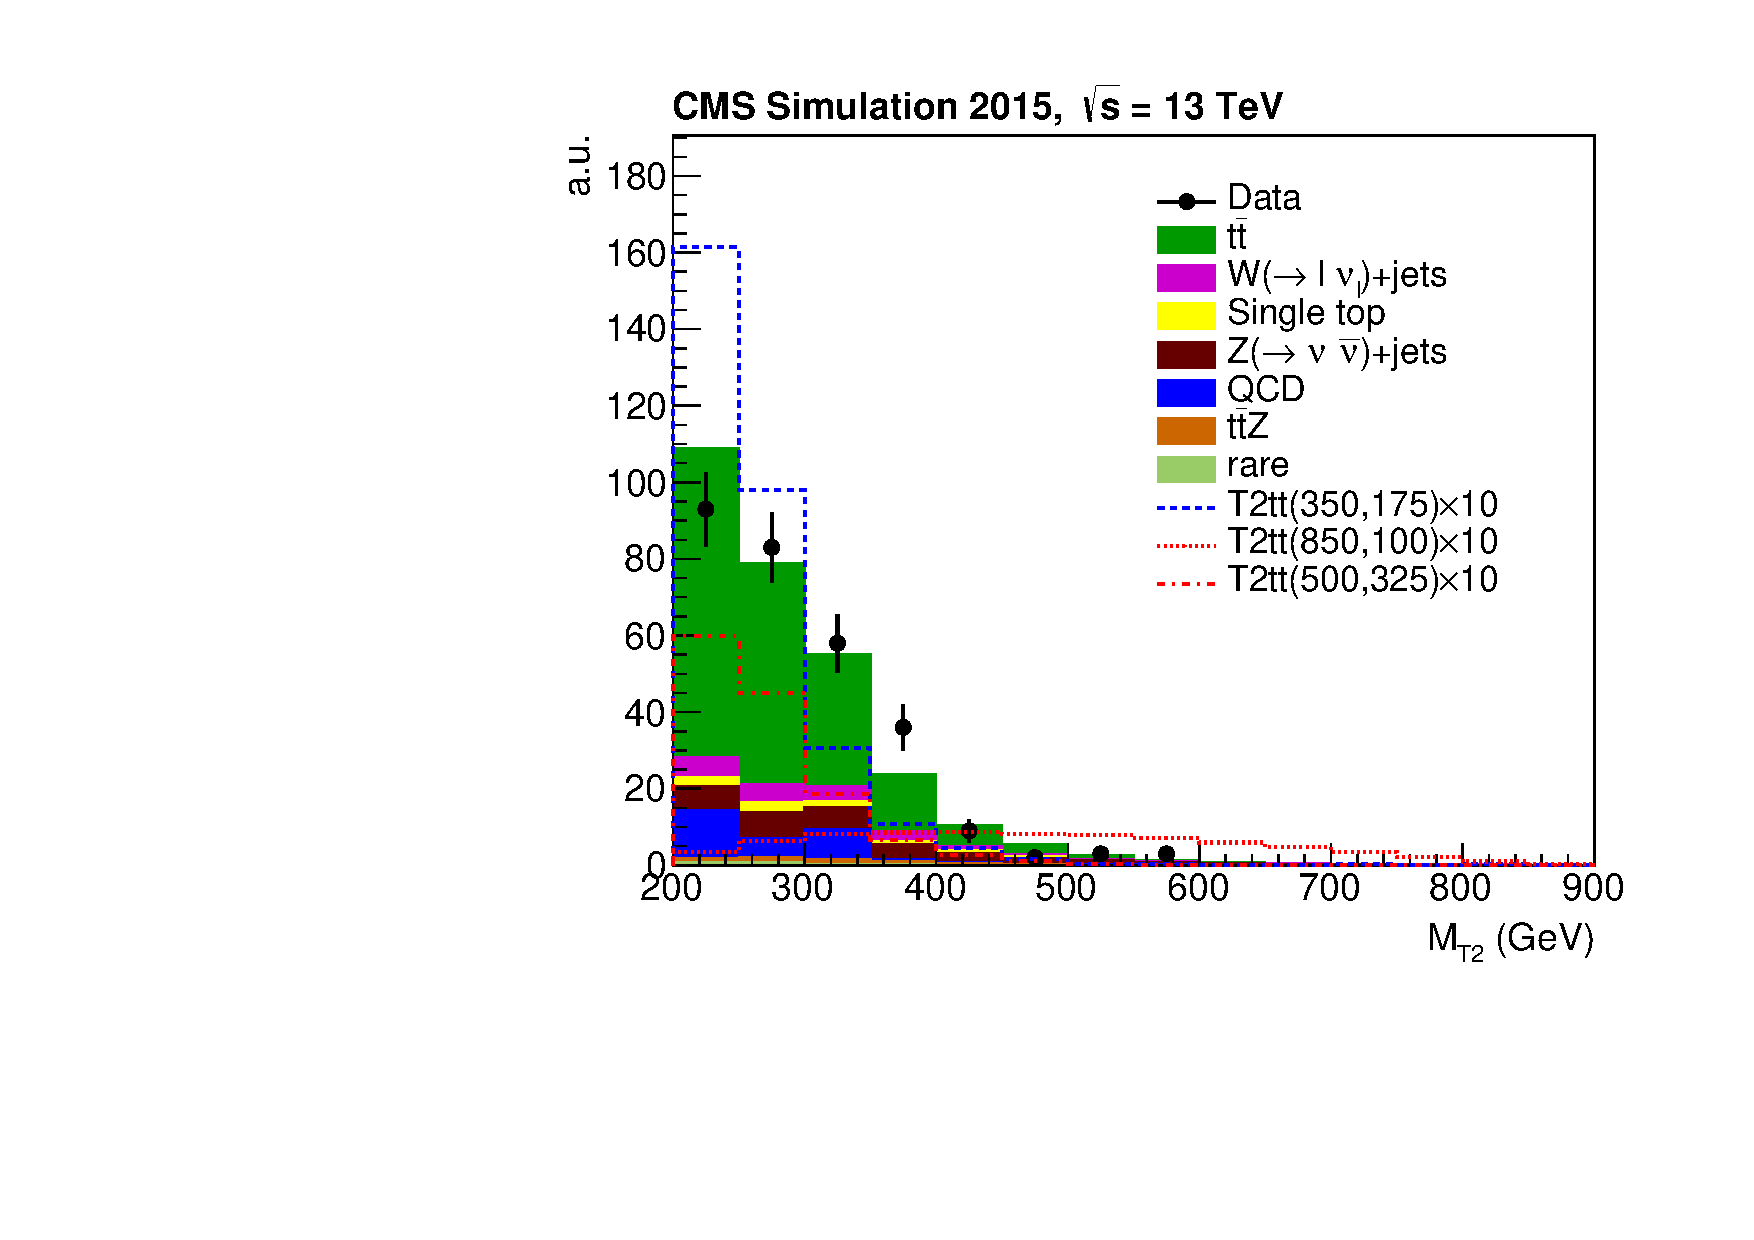
\includegraphics[width=0.48\linewidth]{figures/comb_MT2_baseline.pdf}
    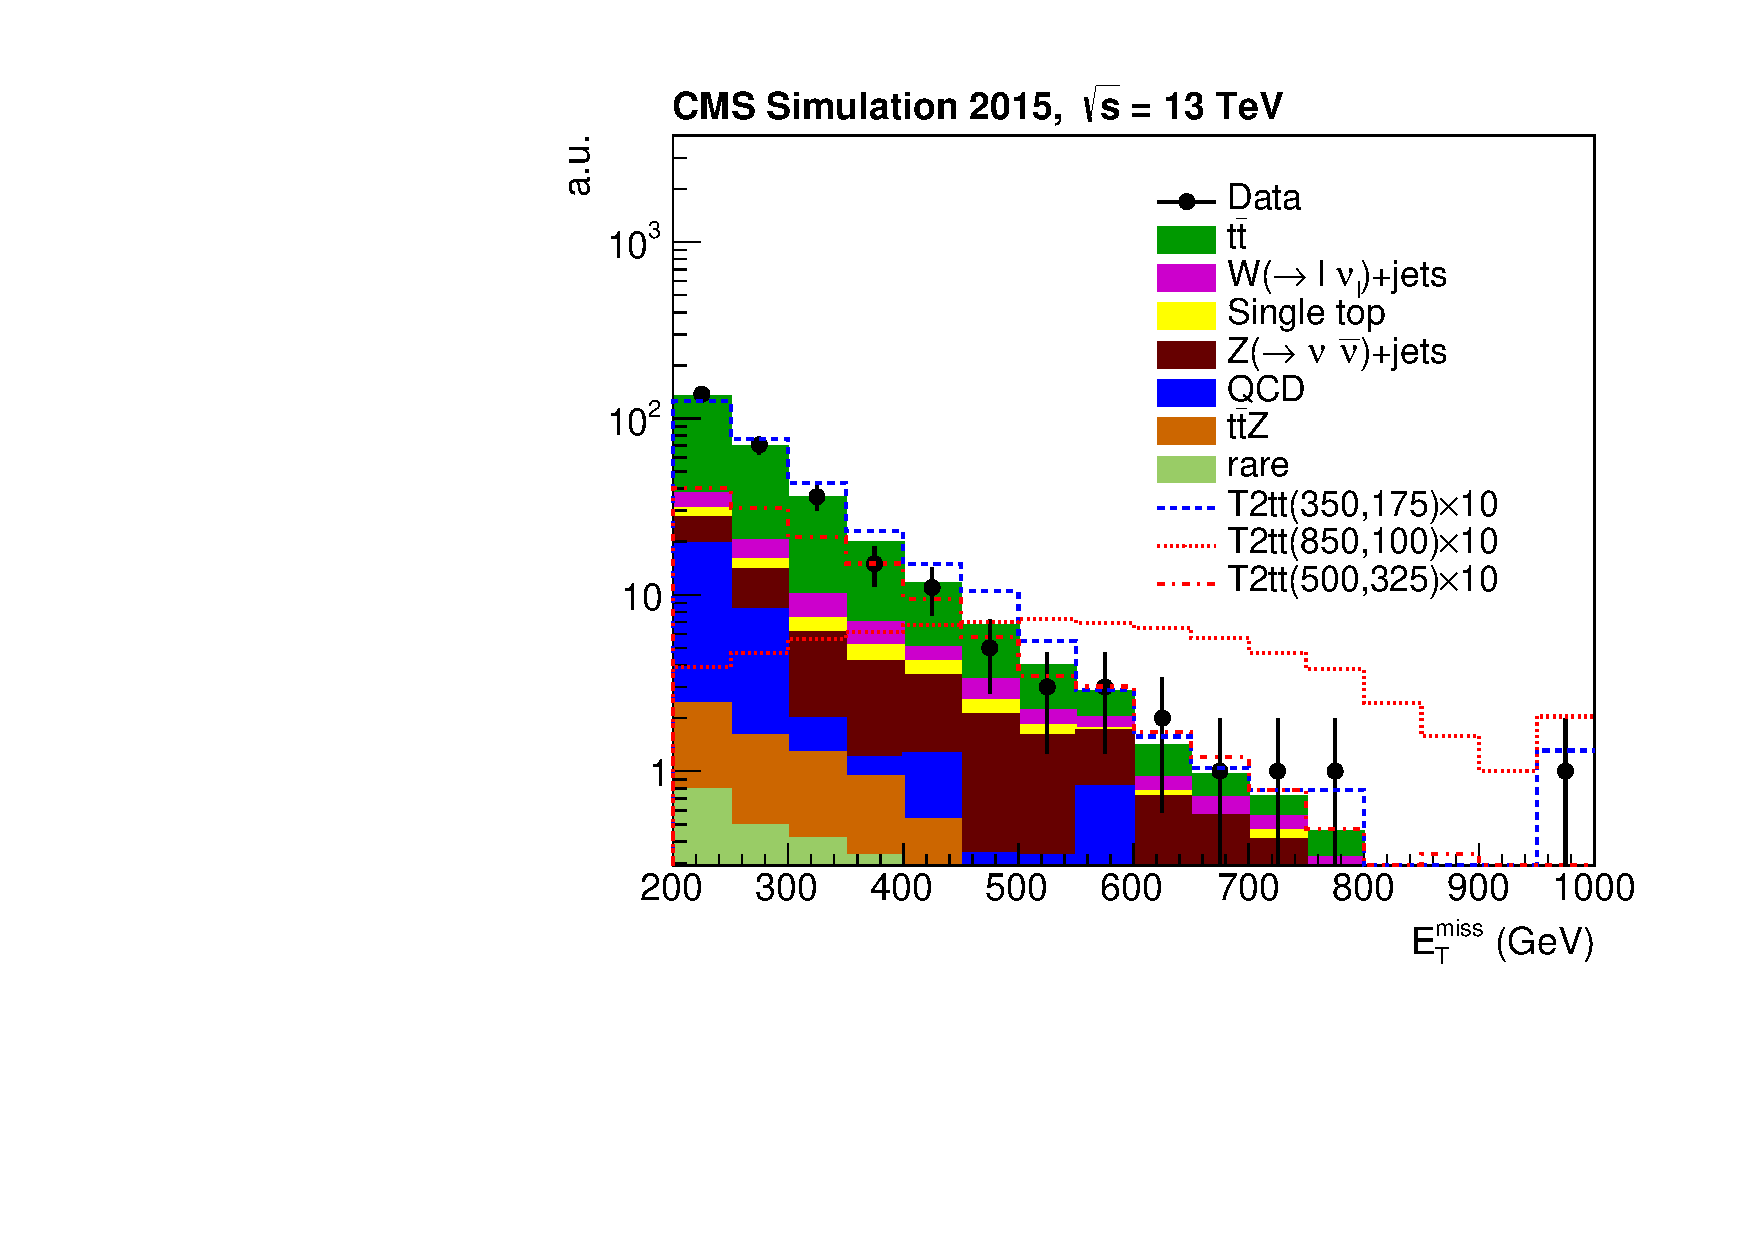
\includegraphics[width=0.48\linewidth]{figures/comb_met_baseline.pdf}
    \caption{ Comparison of the distributions between total SM backgrounds from simulation and several signal points for \ntops, \nbjets, \MET and \MTTwo clock-wise. }
    \label{fig:compSBvars}
  \end{center}
\end{figure}
%%%%%%%%%%%%%%%%%%%%%%%%%%%%%%%%%%%%%%%%%%%%%%%%%%
The search bins defined after pre-selection cuts are illustrated in Fig.~\ref{fig:SBXX}. 
%%%%%%%%%%%%%%%%%%%%%%%%%%%%%%%%%%%%%%%%%%%%%%%%%%
\begin{figure}[h]
  \begin{center}
    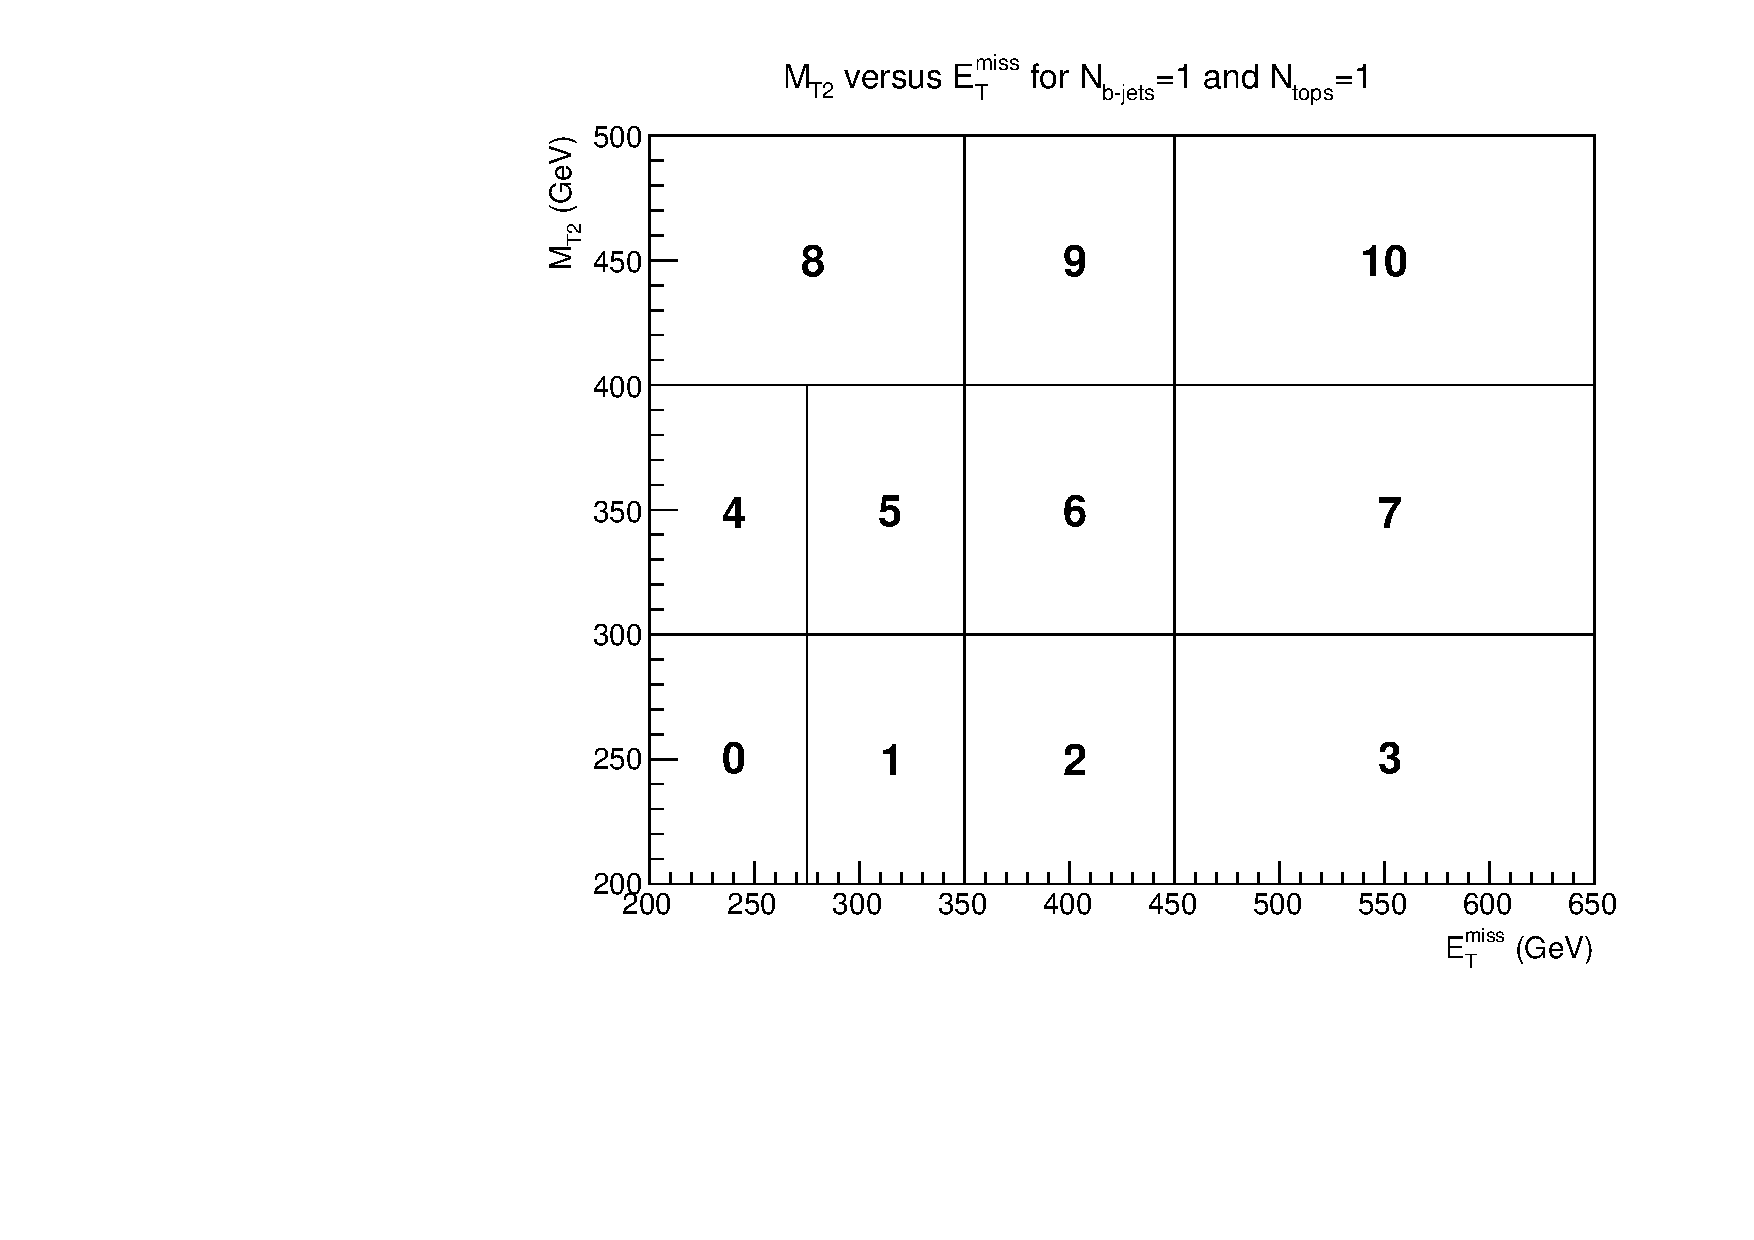
\includegraphics[width=0.45\linewidth]{figures/poly_MT2_vs_met_merged_0.pdf}
    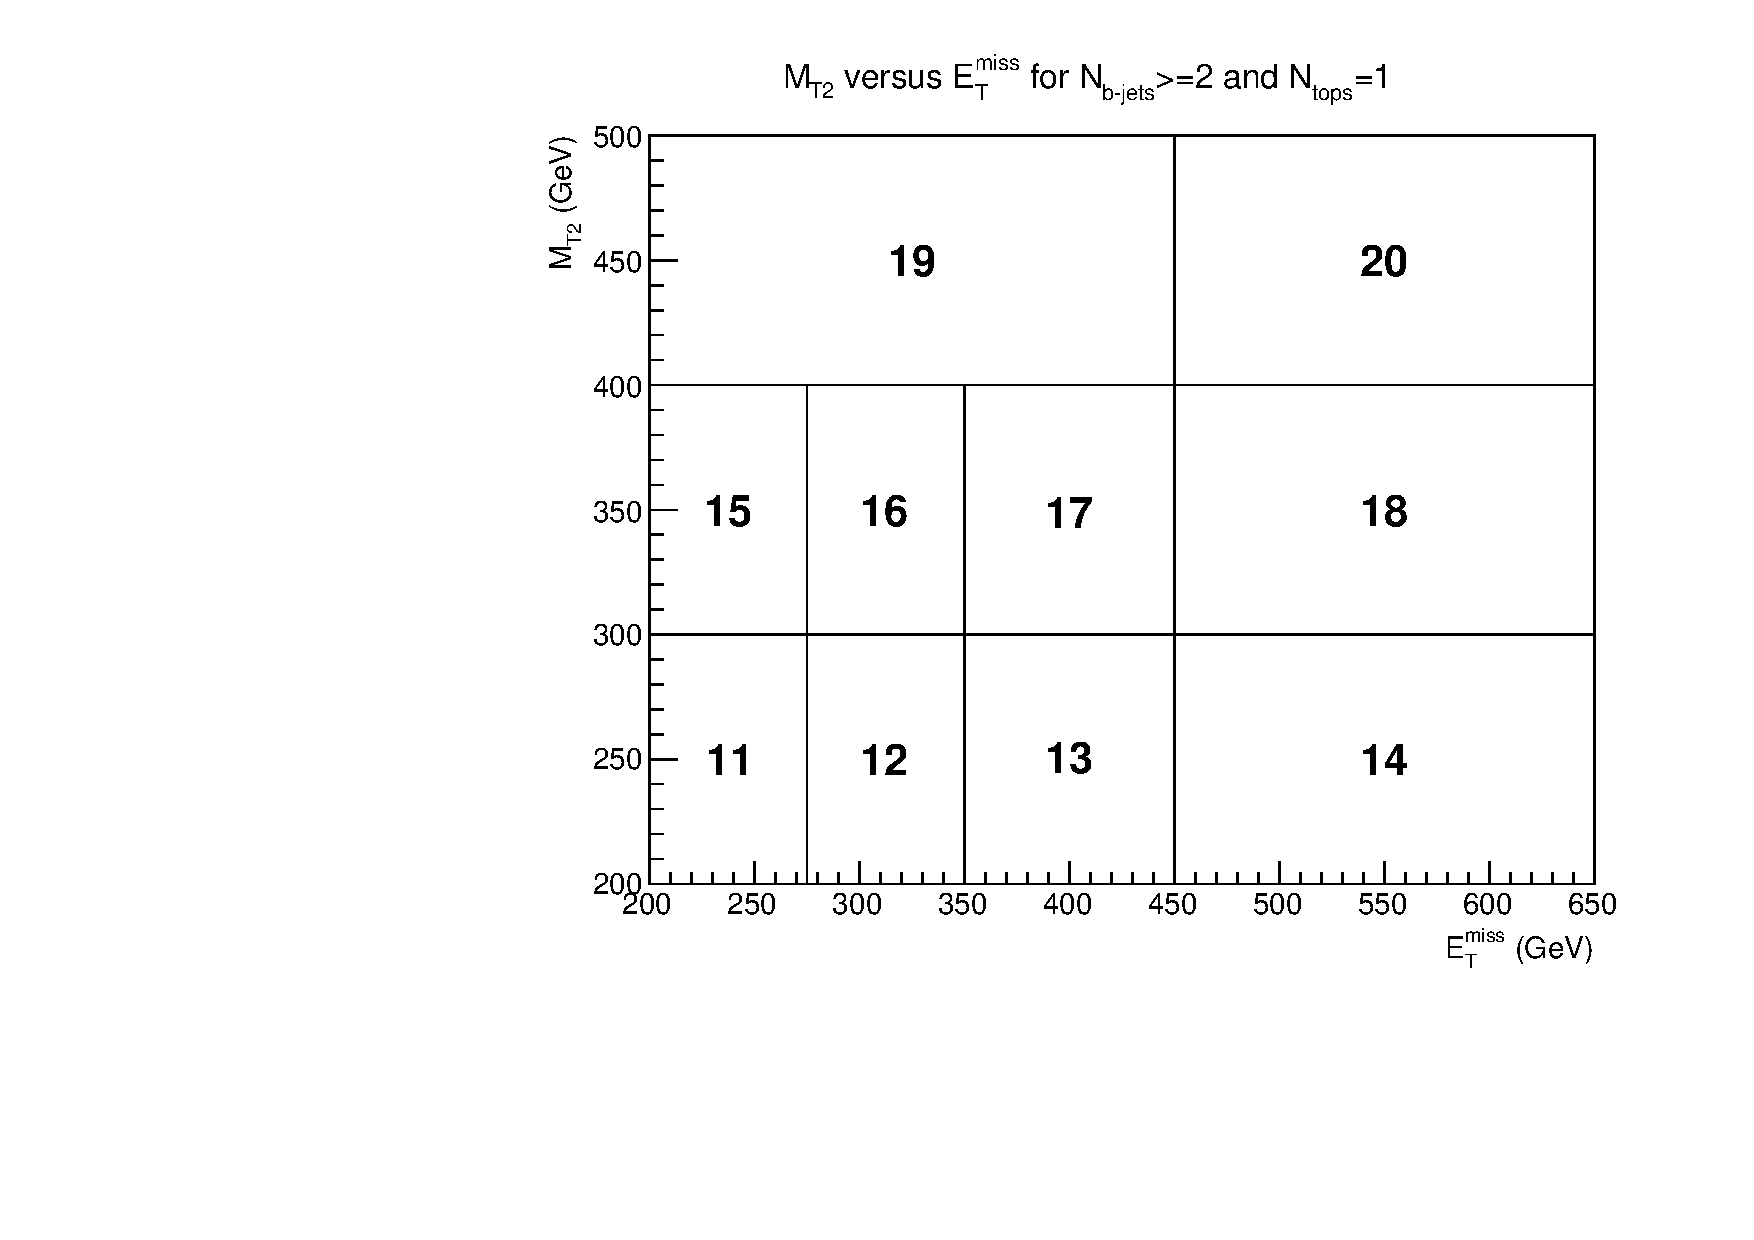
\includegraphics[width=0.45\linewidth]{figures/poly_MT2_vs_met_merged_1.pdf} \\
    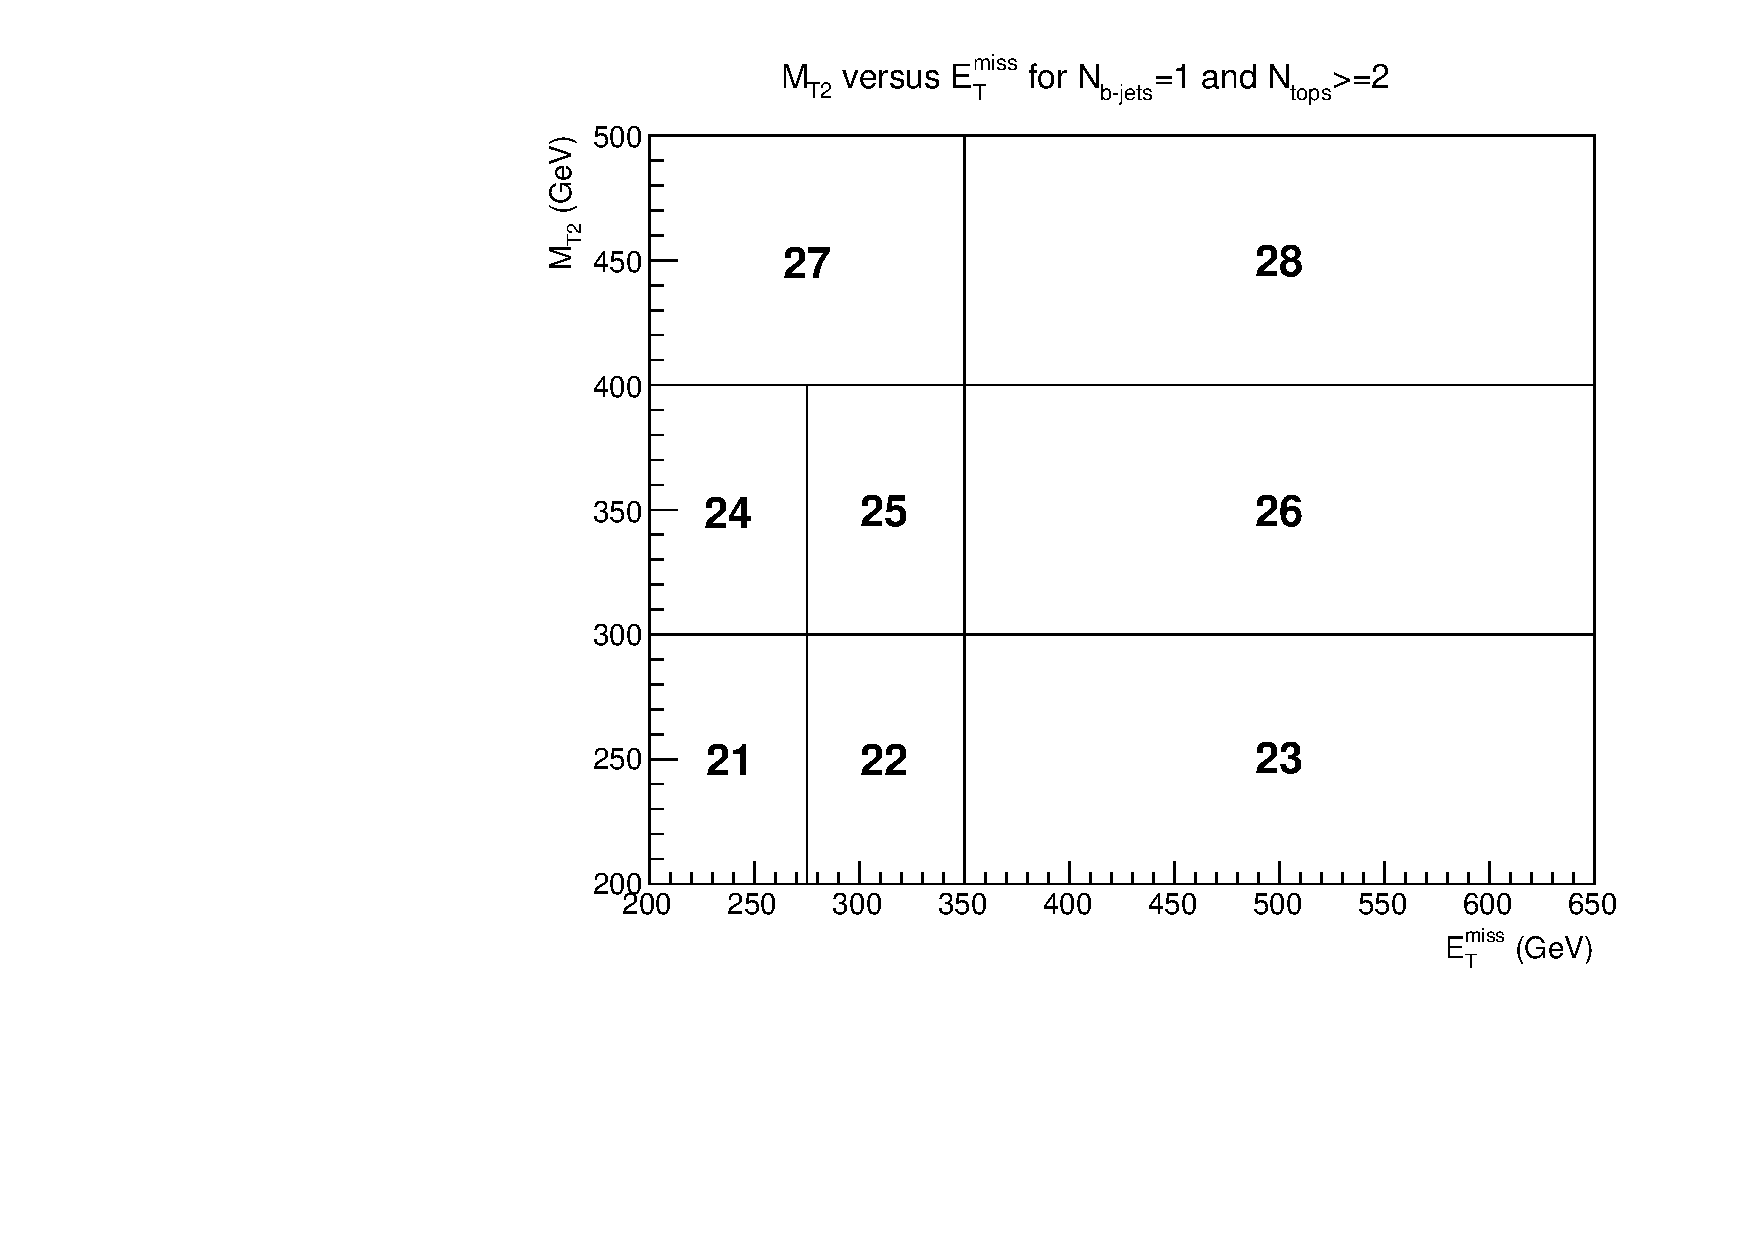
\includegraphics[width=0.45\linewidth]{figures/poly_MT2_vs_met_merged_3.pdf} 
    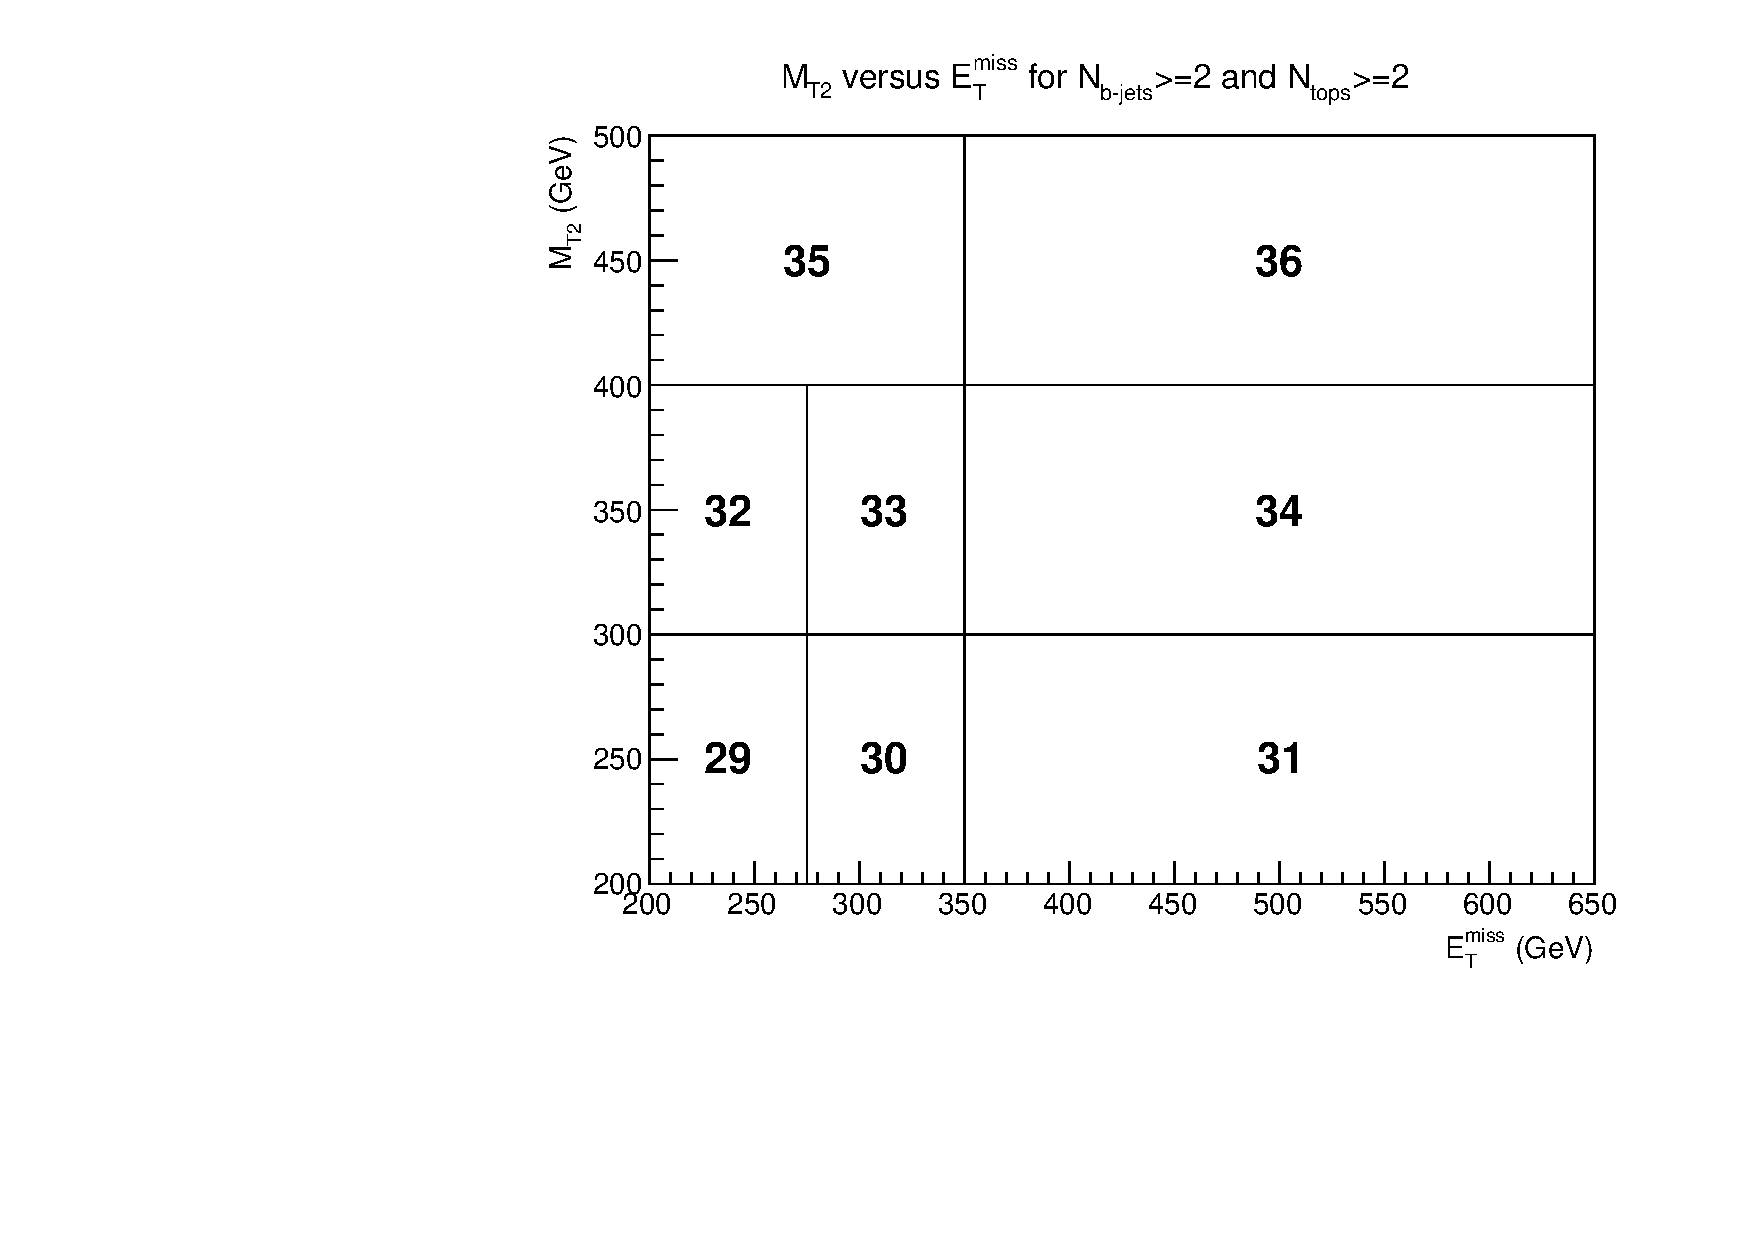
\includegraphics[width=0.45\linewidth]{figures/poly_MT2_vs_met_merged_4.pdf} \\
    \caption{ Search bin definitions after pre-selection cuts. }
    \label{fig:SBXX}
  \end{center}
\end{figure}
%%%%%%%%%%%%%%%%%%%%%%%%%%%%%%%%%%%%%%%%%%%%%%%%%%
The numbers displayed in the figures are the binning indices which are used throughout the analysis.


%%%%%%%%%%%%%%%%%%%%%%%%%%%%%%%%%%%%%%%%%%%%%%%%%%
\subsection{Monte Carlo simulated event samples}
%%%%%%%%%%%%%%%%%%%%%%%%%%%%%%%%%%%%%%%%%%%%%%%%%%

%-------------
The analysis uses a set of Monte Carlo (MC) samples for background estimation method development and predictions as well as SUSY signal samples for interpretation of the results in the light of a number of simplified models. The {\MADGRAPH}5~\cite{Alwall:2011uj} event generator is used to simulate \ttbar, \wjets, \zjets, and QCD multijet events.
%
Single-top events in the $t$ and $\cPqt\PW$ channels are described using the \POWHEG v1.0~\cite{Nason:2004rx,Frixione:2007vw,Alioli:2010xd,Alioli:2009je,Re:2010bp} program, and in the $s$ channel using the {\MADGRAPH}5{\textunderscore}a{\MCATNLO}~\cite{Alwall:2014hca} program. 
%
The latter generator is also used to simulate events with dibosons ($\PW\PW$, $\cPZ\cPZ$, and $\PW\PH$ production, etc., with $\PH$ a Higgs boson) and rare processes ($\ttbar\PW$, $\ttbar\cPZ$, and $\PW\PW\cPZ$ combinations, etc.), except that \POWHEG~\cite{Melia:2011tj} is used for $\PW\PW$ events in which both {\PW} bosons decay leptonically.
%
Simulation of the detector response is based on the \GEANTfour~\cite{Agostinelli:2002hh} package. 
%
All cross sections come from calculations performed at next-to-next-to-leading-order (NNLO), unless otherwise noted.  
%
All simulated samples include pile-up with an average of 20 interactions per bunch crossing and a 25~ns interval between bunches.
%-------------
Signal T2tt and T2tb events are simulated for a range of stop \mstop LSP \mlsp mass values, with $\mlsp<\mstop$.
%
The signal samples are based on the \MADGRAPH generator, with up to two partons present in addition to the stop pair. 
%
The decays of the stop are described with a pure phase-space matrix element~\cite{Sjostrand:2014zea}. 
%
The signal production cross sections are computed~\cite{bib-nlo-nll-01,bib-nlo-nll-02,bib-nlo-nll-03,bib-nlo-nll-04,bib-nlo-nll-05} with next-to-leading order (NLO) plus next-to-leading-logarithm (NLL) accuracy. 
%
To reduce computational requirements, the detector is modeled with the CMS fast simulation program~\cite{Orbaker:2010zz,bib-cms-fastsim-02}, which yields consistent results compared with the {\GEANTfour}-based simulation.
%-------------
The NNPDF3.0LO~\cite{Ball:2014uwa} parton distribution functions (PDF) are used for the \MADGRAPH signal and background samples, and the NNPDF3.0NLO~\cite{Ball:2014uwa} PDFs for the \POWHEG and {\MADGRAPH}5{\textunderscore}a{\MCATNLO} samples. 
%
All simulated samples use the \PYTHIA 8.2~\cite{Sjostrand:2014zea} program to describe parton showering and hadronization.
